\documentclass[conference]{IEEEtran}
\IEEEoverridecommandlockouts
% The preceding line is only needed to identify funding in the first footnote. If that is unneeded, please comment it out.
\usepackage{cite}
\usepackage{amsmath,amssymb,amsfonts}
\usepackage{algorithmic}
\usepackage{graphicx}
\usepackage{textcomp}
\usepackage{xcolor}
\usepackage{minted}
\usepackage{dirtree}
\usepackage{pgfplots}
\usepackage{hyperref}
\usepackage[english]{babel}
\def\BibTeX{{\rm B\kern-.05em{\sc i\kern-.025em b}\kern-.08em
    T\kern-.1667em\lower.7ex\hbox{E}\kern-.125emX}}
\begin{document}

\title{Ansible: a Software Architecture Analysis}

\author{\IEEEauthorblockN{Simone Berni}
\IEEEauthorblockA{\textit{Alma Mater Studiorum} \\
Bologna, Italy \\
simone.berni2@studio.unibo.it}
}

\maketitle

\begin{abstract}
This document explains how Ansible is designed, what are the drivers behind the software and how these requirements are converted in a simple but powerfull architecture, with a focus on its components and the relation between them. 
\end{abstract}

\section*{Introduction}
The paper structure is the following: first of all, in section \ref{ansible} is discussed what is Ansible, how it works and for whom was designed. After that, in section \ref{context}, the drives behind Ansible are described, in the form of Uitlity tree, user cases and non functional requirements. The section \ref{structure} is used to describe the main components of Ansible, the relations between them, the data flow inside the application and why Ansible developers have chosen this architecture. In section \ref{analysis} are discussed pro and cons of this type of architecture and what could have be done to upgrade it. Last section is \ref{similar}, where are described similar architectures and the differences between them.

\section{Ansible} %description
\label{ansible}
Ansible is a tool that provides reliability, consistency and scalability to your infastructure. It is an IT automation engine that improves cloud provisioning, configuration management, application deployment and databases configuration.\\
It makes sure that all the necessary packages and all other software that are needed to run the applications are present and updated on the node.\\
It holds all the historical data of your application, so the devops engineer is easily able to roll back to a previus version, or to upgrade to a newer one.\\
It does not use additional infrastructure, making it simple to deploy, is agentless, unlike its competitors, so it does not require any particular software on the nodes to manage them.\\
The configuration is given using a very simple language, YAML, in the form of Playbook, allowing to describe the automation jobs in pretty much plain English.\\ 
Ansible il built on top of \textbf{Python}, one of the most used programming language in today's world, making its installation requirements pretty much not existing.\\ 
Each job is pushed to the clients machines via \textbf{SSH}, a secure network authentication protocol, that can be considered passwordless if you previusly exchanged the keys. \\
There are two main components inside ansible automation engine: the \textbf{Inventory} and the \textbf{Playbook}.
Both are just Yaml files, but the first is used for list hosts and groups that needs to be configured, aliases and variables for the playing.\\
The latter instead defines what has to be done in the nodes: it is a list of plays, and each play contains different tasks, each task includes modules, that can be one of the hundreds of inbuilt modules, or a new one created from the user.\\
The language used for its configuration is easily readable and trasparent, even if the engineer doesn't have a programming background, because the automation code should make perfect sense to the administrator even after years, without having to remember another syntax or how to describe some features.\\
If the many features aren't enough for someone needs, is easy to extend Ansible with your own modules and plugins. Modules, for example, just need to return a JSON file, and they can be written in any programming language. There are also varius API for extending the connection types, for example if you don't want to use SSH to transmit your payload,or the use of callbacks and even the possibility to add new server side behaviors.\\

\section{Context}
\label{context}
\subsection{Scope}
The main feature of Ansible is the capacity to \textbf{Orchestrate} very heterogeneous system: is possible to install the same software on many different machines, each one with a different OS, without the need of any kind complex syntax, because Ansible will abstract the concept and will manage internally what package manager has to be used in which OS, and even which other software are prerequisites for the application.\\ 
Is important to understand for who the software was designed: people that have to manage very large, heterogeneous and complex systems, and want to describe every operation, every managemnt aspect of their infrastructure without making irreversible errors.\\
Every \textit{DevOps engineer} that care about their role will probably learn to use Ansible in their lifetime. 

\subsection{Use Cases}
It's possibile to split the uses cases in three categories: how to configure Ansible, how to manage the nodes of an infrastructure, and how to record what has be done.\\
\begin{table}[htbp]
\begin{center}
\begin{tabular}{|p{0.6cm}|p{1.4cm}|p{5cm}|}
\hline
\textbf{Use Case} &\textbf{Description}&  \textbf{Scenario} \\
\hline
\hline
UC1 & Manage Users & Every node of the infrastructure has the same set of users and every user is able to log in every machine. \\
\hline
UC2 & Install Application & Every node of the infrastructure should be able to install the same software, even if the machines have different OS, packet manager and configurations. \\
\hline
UC3 & Provide reports & Whenever the nodes in the network are modified via Ansible, a report of what has be done, what was sucessfull and what not, has to be created.   \\
\hline
UC4 & History and Downgrade & For each node of the infrastructure the administrator has to be able to see its history and has to be able to downgrade the system to a previus version.\\
\hline
UC5 & Configuration Syntax & The syntax has to be easy to remember and to understand, since the administrator wants to focus on what has to be done, not how to write it.  \\
\hline
UC6 & Manage Cloud & The user should be able to use Anisble to manage many Amazon AWS instances.  \\
\hline
UC7 & Extendable & If the builtin modules doesn't answer a user problem, should be easy to create and integrate a new custom module. \\
\hline
UC8 & Secure Connection & The sensible data should travel in a secure communication channel to the nodes. \\
\hline
\end{tabular}
\label{tab1}
\end{center}
\end{table} 
\newpage
\section{Non Functional Requirements}
The main non functional requirements that have been found during the Ansible analysis are described in figure \ref{utility}. Is possible to see how they are related to the uses cases, in the following table.
\begin{table}[htbp]
\begin{center}
\begin{tabular}{|p{1cm}|p{1.5cm}|p{3cm}|p{1.2cm}|}
\hline
\textbf{Id} &  \textbf{Requirement} & \textbf{Scenario} & \textbf{Associated Use Cases} \\
\hline
\hline
NF1 & Usability & The application should be able to configure three nodes easier and faster than manually & UC1 \\
\hline
NF2 & Usability & The application should be able to configure any part of the system using the same syntax structure & UC1, UC2, UC5 \\
\hline
NF3 & Modifiability & The application should allow the creation of any kind of custom modules & UC7 \\
\hline
NF4 & Efficiency & The application should be able to configure a medium size network(15 nodes) in under 2 minute & UC6 \\
\hline
NF5 & Interoperability & The application should work the same with Cloud and intranet network & UC6 \\
\hline
NF6 & Security & The application should be able to connect to the nodes via SSH & UC8 \\
\hline
NF7 & Security & The application should be able to encrypt sensible data in a secure way & UC8 \\
\hline
NF8 & Operability & The application should store the history for each node forever & UC4\\
\hline
NF9 & Scalability & The application should work with at least 50 nodes without losing performance & UC2, UC6 \\
\hline
\end{tabular}
\label{tab2}
\end{center}
\end{table} 
\begin{figure}[h]
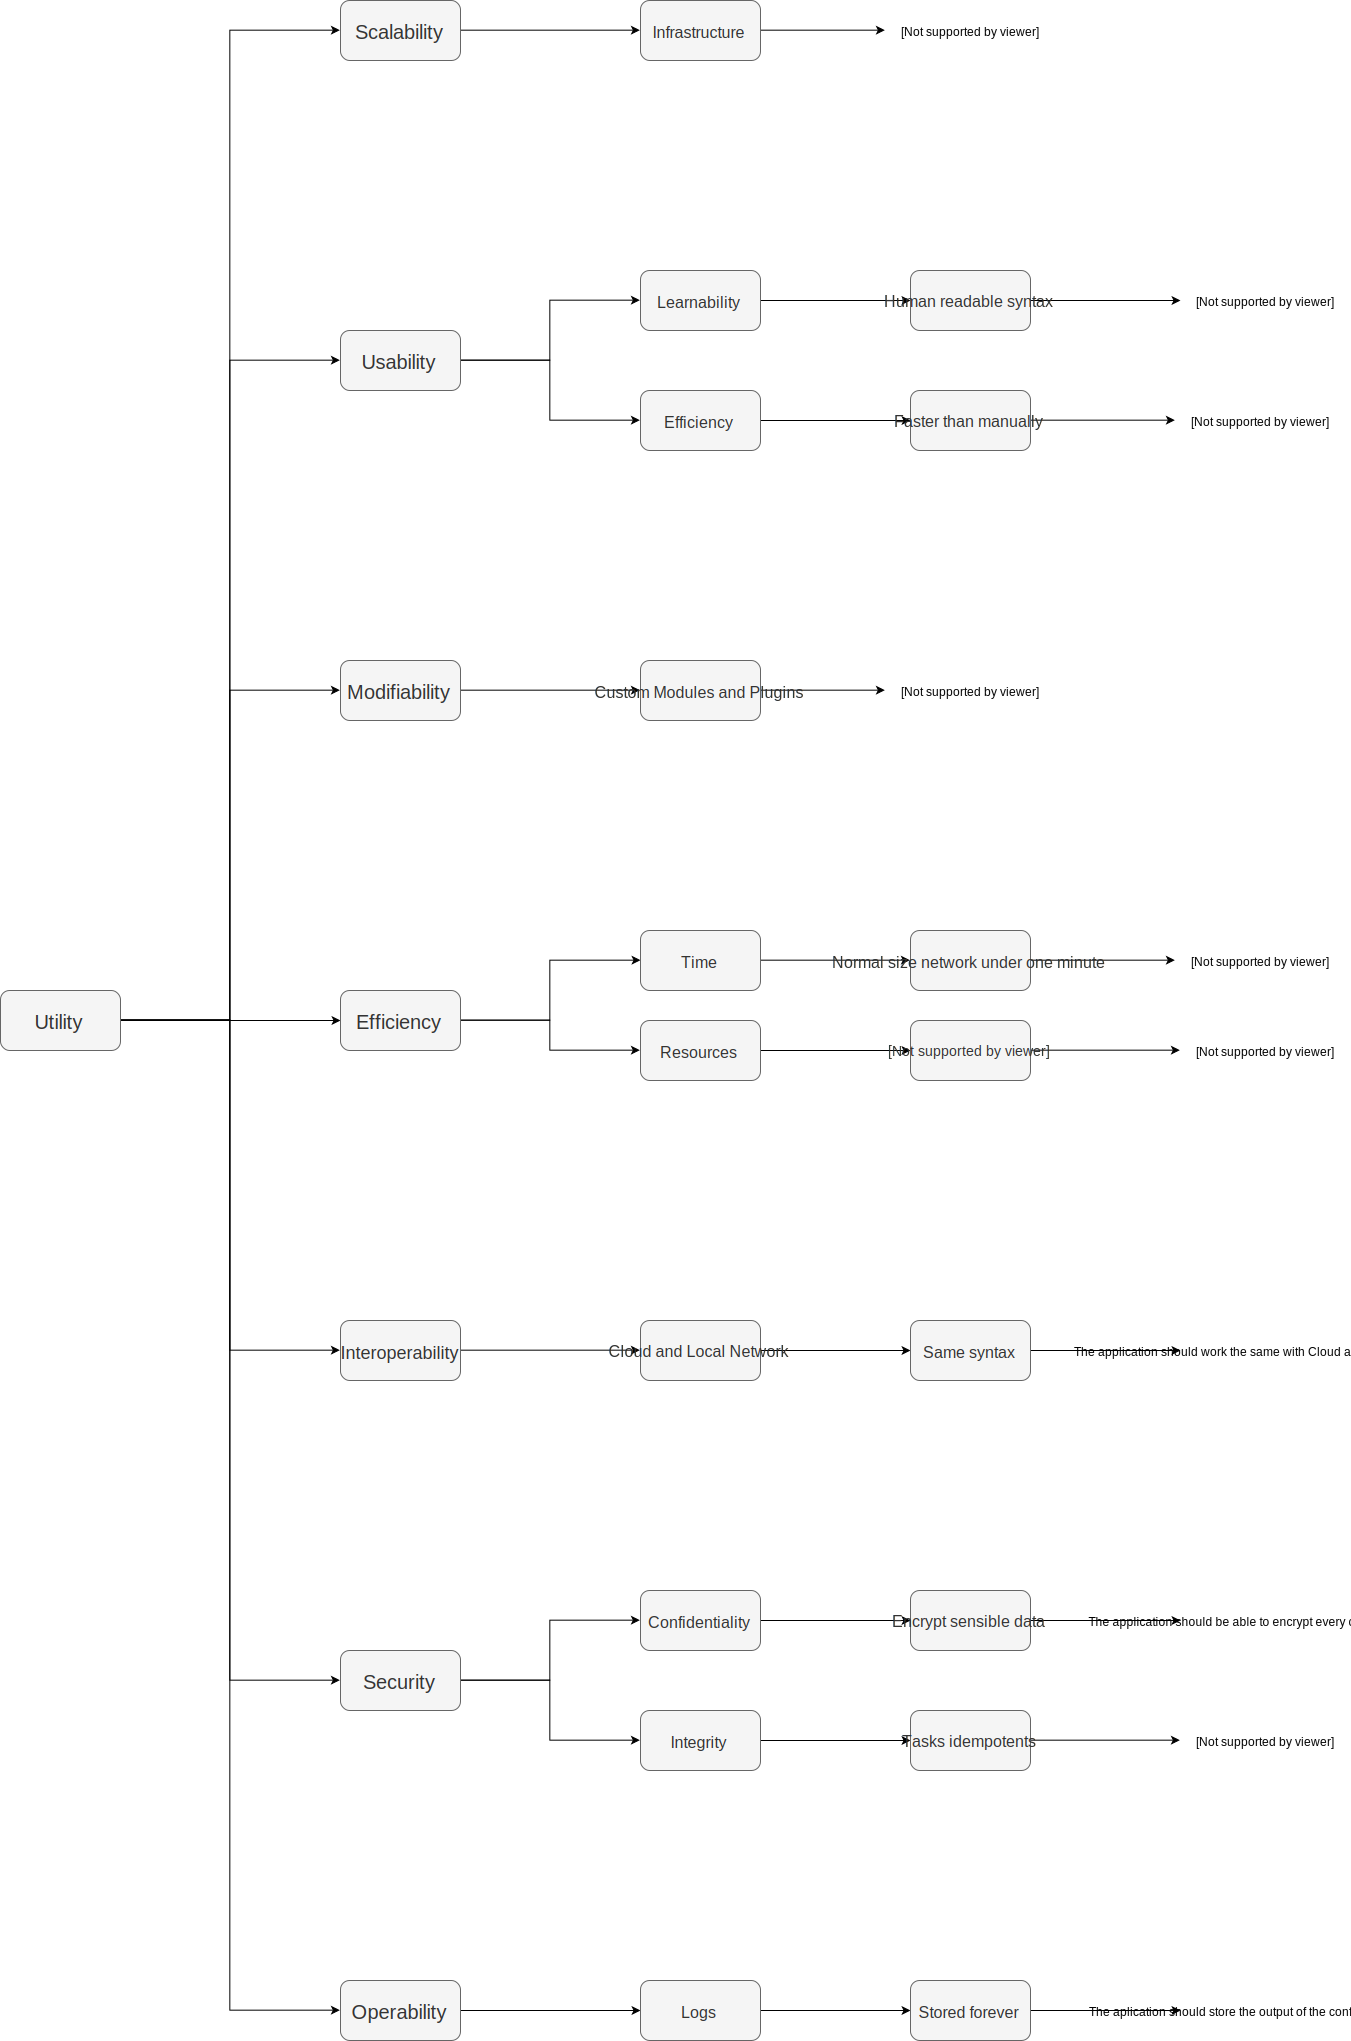
\includegraphics[width=0.48\textwidth]{UtilityTree.png}
\caption{Utility tree}
\label{utility}
\end{figure}
\section{Structure Analysis}
\label{structure}
The Ansible structure is not a complicate one, because its main goal is to reduce deployment time and resources for its users, and let them focus on their orchestration work. The main components are 4: the \textbf{Inventory}, where the hosts and the groups are defined; the \textbf{Module}, a program that is used to accomplish a task; the \textbf{Vault}, used for encrypt sensible data; the \textbf{Playbook}, the kernel of this system, where what has to do, against who and in which way, is defined.\\
\begin{figure}[h]
\includegraphics[width=0.48\textwidth]{Schema.jpg}
\caption{Ansible structure}
\end{figure}
\newpage
\subsection{Component Analysis}
\subsubsection{Inventory}
Ansible works against multiple managed nodes or “hosts” in your infrastructure at the same time, using a list or group of lists known as inventory. Once your inventory is defined, you use patterns to select the hosts or groups you want Ansible to run against for each task.\\
In figure \ref{inventory} is possible to see an example of an inventory file.\\
\begin{figure}[h]
\begin{minted}[
    frame=single,
  ]{yaml}
 all:
  hosts:
    mail.example.com:
  children:
    webservers:
      hosts:
        foo.example.com:
        bar.example.com:
    dbservers:
      hosts:
        one.example.com:
        two.example.com:
        three.example.com:
    east:
      hosts:
        foo.example.com:
        one.example.com:
        two.example.com:
    west:
      hosts:
        bar.example.com:
        three.example.com:
    prod:
      children:
        east:
  \end{minted}
  \caption{Inventory example}
  \label{inventory}
\end{figure}\\
Is possible to use multiple inventory at the same time, or to pull them, for example, from cloud sources, and work with dynamic inventories, usefull if you do not want to replicate the same inventory in more playbooks. Ansible has developted the \textit{Inventory Plugins} to work with the latter: the script is called at runtime to discover real-time inventory data.\\
Another use of the inventory component is to assign a value to a variable, for a later use in the playbooks, or for aliases.\\
The Ansible goal is to write automation code that is readble after years from it's preparation: this is why is common to organize different groups in different files. It is even possible to create a directory named after each group, and in this case Ansible will read each file in these directories in lexicographical order.\\
An example of a filesystem of a standard inventory is in figure \ref{dirtree}.\\
\begin{figure}[h]
\framebox[0.5\textwidth]{%
\begin{minipage}{0.5\textwidth}
  \dirtree{%
  .1 /etc/ansible/.
  .2 hosts.
  .2 hosts\_var/.
  .3 DisiLab.
  .2 group\_vars/.
  .3 web\_servers.
  .3 datacenters.
  .3 \vdots.
  }
\end{minipage}
}
\caption{Inventory dirtree}
\label{dirtree}
\end{figure}
\subsubsection{Module}
The Ansible modules are just small programs, a  \textbf{task}, that describe the desired state of the system. They are pushed to the nodes of the infrastructure, executed over SSH, and then removed from the system, using the \textit{ControlPersist} feature of SSH.\\
Technically Ansible opens 3 SSH connections: the first creates a temporary folder, the second is used for copying the module payload from the source to the node, and the third has to execute the script, to remove the directory and to capture the module results in a JSON format. The only costraint on how the module has to work is its output format, that must be JSON, but they can, and they are, written in any programming language.\\
Is even possible to reduce the number of SSH connection using a feature called \textit{pipelining}: Ansible will open an SSH connection and start a Python interpreter on the remote host, and in this connections are piped the module payload for its execution.\\
To doing so Ansible must install, if it is not present, Python on each remote host.\\
Each module has three possible output:
\begin{itemize}
    \item \textbf{ok}: the module completed its task
    \item \textbf{changed}: the module had to make changes to the system
    \item \textbf{failed}: the module did not complete its task
\end{itemize}
Is possible to use a module in two ways: directly from the command line, if there is the need to execute a single task in many nodes just one time, without having a proper configuration, or inside a Playbook, if there is the desire to create a more complex orchestration between the nodes.\\
An example of module using YAML syntax is in figure \ref{restartsever}.\\
\begin{figure}[h]
\begin{minted}[
    frame=single,
  ]{yaml}
 - name: restart webserver
    service:
    name: httpd
    state: restarted
  \end{minted}
  \caption{Restart a webserver}
  \label{restartsever}
\end{figure}\\
Since Ansible has to be fast to deploy, there are many builtin modules offered to its users:
\begin{itemize}
    \item Cloud modules
    \item Clustering modules
    \item Commands modules
    \item Database modules
    \item Monitoring modules
    \item Network modules
    \item Packaging modules
    \item ...
\end{itemize}
The modules are part of the Ansible Core, and there is no need of daemons, databases or servers, since they are installed with Ansible.
Since they are pushed via SSH, the hosts machines do not require any kind of configuration, differently from its competitor.\\
If no one of the existing modules cover the functionality that the user needs, is possible to develop a new module. But should the user develop a module?\\ Since Ansible is opensource and its code is on Github, an existing Pull Request may cover the functionality needed, and it's a good point from where to start to the development. Maybe the functionality is a combination of others modules, and in this case is enough to combine them and create a \textbf{Role}.\\
A role in Ansible is one of the many way to group modules, hiding implementation details and creating a new level of abstraction.\\

\subsubsection{Vault}
Ansible Vault is a feature that allows users to keep sensitive data, such as passwords, keys and tokens, in encrypted files rather than plaintext.\\
Each structured data file that can be used by Ansible, like the inventory file, is possible to encrypt via Vault. Is even possible to have a variable-level encryption, in this way a file can still be readble, encrypting only the password.\\ At the same time is important to remember that is not necessary to encrypt everything, but as best practice only the smallest amount of data possible.\\
The Vault offers many utilities to work with file and encryption:
\begin{itemize}
    \item Create a new encrypted file
    \item Edit a encrypted file
    \item Encrypt an unecrypted file
    \item Rekeying encrypted file
\end{itemize}
The password for unlock the Vault can be given via prompt, or password manager like \textit{pass}.

\subsubsection{Playbook}
Playbooks are Ansible's configuration, deployment, and orchestration language. Every other component listed before works together inside a Playbook. \textit{The Playbook is like an instruction manual, where the \textbf{inventory} hosts are the material, the \textbf{modules} are the tools and the \textbf{vault} the cabinet}.\\
Playbooks are designed to be human-readable and there are many different way to organize tasks to obtain the same result.\\
Like the inventory, Playbooks are expressed in YAML format, because Ansible intentionally tries to not be a programming tool, but rather a configuration one, and it doesn't want that the engineer using it has to learn another language.\\
The structure of a Playbook is quite simple at start: is just one or more \textbf{play} in a list. In figure \ref{playbook} is possible to see an example.
\begin{figure}
\begin{minted}[
    frame=single,
  ]{yaml}
---
- hosts: webservers
  remote_user: root

  tasks:
  - name: apache latest version
    yum:
      name: httpd
      state: latest
  - name: write the apache config file
    template:
      src: /srv/httpd.j2
      dest: /etc/httpd.conf

- hosts: databases
  remote_user: root
  become: yes
  become_method: sudo
  tasks:
  - name: postgresql latest version
    yum:
      name: postgresql
      state: latest
  - name: postgresql is started
    service:
      name: postgresql
      state: started

  \end{minted}
  \caption{A playbook with two plays}
  \label{playbook}
\end{figure}
The first play check that apache is at the latest version and create a config file for each hosts in the group webservers.
The second play check that postgresql is at the latest version and that is started for each hosts in the group databases.\\
The \textit{hosts} line is a list of one or more groups or hosts. The hosts are created during the inventory phase.
\textit{Remot\_user} is the name of the user account used for the task. Inside the tag \textit{tasks} are listed each module that will be used. In the first play, for example, are used the modules \textit{yum} and \textit{template}. the \textit{become} keyword is used to execute the task as another user, default as root, and \textit{become\_method} describe which privilege escalation method should be used.\\
Each task is executed against all machines in the hosts patttern before moving on with the next task. \\
One note that must be said on the Playbook is that it should be idempotent: running the same Playbook more than once should be safe, and to be that, each play and each task have to be idempotent. This is done by simply checking that the desidered final state is already achieved or not.\\
Playbooks files will grow with the complexity of the system and the number of tasks that must be performed. With Ansible there is the possibility to \textit{include} and \textit{import} Playbooks, allowing the possibility to break up a large file into smaller ones, which can be used across multiple parent playbooks. The differences between the two methods is that the \textit{include} keywords refers to dynamic inclusion, and \textit{import} to static. More deeply, the differences between static and dynamic is that the first one is pre-processed by Ansible during the parsing time, the latter during runtime.\\
Variables normally are defined inside the inventory space, but is still possibile to define them directly in a Playbook. For using them, the standard way is with the Jinja2 templating system, commonly used in Python packages. A common softare that uses Jinja2 templating is, for example, \textbf{Flask}.\\

\begin{figure}[h]
\begin{minted}[
    frame=single,
  ]{yaml}
  task:
  - name: write the apache config file
    template:
      src: "{{local_path}}}httpd.j2"
      dest: "{{remote_path}}httpd.conf"
  \end{minted}
  \caption{Jinja2 templating}
\end{figure}
Inside the templating is possible to have access to only the variables that are in scope for a host.\\
Is even possible to discover variables, speking directly with the remote system. This type of variables are called \textbf{Facts}, and they all start with \textit{ansible\_} prefix. Figure \ref{facts} is a small example of facts that can be retrieved.\\
\begin{figure}[h]
\begin{minted}[
    frame=single,
  ]{yaml}
{
    "ansible_all_ipv4_addresses": [
        "79.52.61.239"
    ],
    "ansible_all_ipv6_addresses": [
        "::ffff:c0a8:5909"
    ],
    "ansible_apparmor": {
        "status": "disabled"
    },
    "ansible_architecture": "x86_64",
    "ansible_bios_date": "11/28/2013",
    "ansible_bios_version": "4.1.5",
    "ansible_cmdline": {
        "console": "ttyS0,115200",
        "no_timer_check": true,
        "nofb": true,
        "nomodeset": true,
        "ro": true,
        "root": "LABEL=cloudimg-rootfs",
        "vga": "normal"
    }
}
  \end{minted}
  \caption{Retrieving facts}
  \label{facts}
\end{figure}\\
Often the result of a play may depend on the value of a variable, a fact, or a previus task output. Inside a Playbook is possible to use conditionals, like the \textit{when} statement, that works exactly like an \textit{if} in a programming languages.\\ 
A simple example is figure \ref{when}:\\
\begin{figure}[h!]
\begin{minted}[
    frame=single,
  ]{yaml}
name: "shut down Arch systems"
command: /sbin/shutdown -t now
when: ansible_facts['os_family']== "Arch"
  \end{minted}
  \caption{When statement}
  \label{when}
  \end{figure}
There is also the \textit{loop} statement, that work exactly as one would expect.\\
Conditionals can be applied inside a task, a roles or hosts, or even during imports.


\subsubsection{Plugin}
Plugins are pieces of code that augment Ansible's core funcionality. Using a plugin architecture is easier for everyone, from the final user to the Ansible developers to add new functionalities.\\
Ansible is shipped with many builtin plugins, for example:
\begin{itemize}
    \item Action Plugins
    \item Become Plugins
    \item Shell Plugins
    \item Connection Plugins
    \item ...
\end{itemize}
When writing a plugin, that are more rules that have to respected compared to writing a module. All plugins must:
\begin{itemize}
    \item Be written in Python
    \item Raise errors
    \item Return strings in unicode 
    \item Be conform to Ansible's configuration and documentation standards
\end{itemize}
Tha programming language must be Python because the \textit{PluginLoader} will load them as Python object that any module can use, and will be executed on the controller side inside a Python interpeter.\\
\newpage

\subsection{Functions}
Each non functional requirement has been resolved inside one or more component. The following table describes this mapping.\\

\begin{table}[htbp]
\begin{center}
\begin{tabular}{|p{0.6cm}|p{1.4cm}|p{5cm}|}
\hline
\textbf{Req} &\textbf{Component}&  \textbf{Description} \\
\hline
\hline
NF1 & Module & Ansible offers enough modules to complete every task that the user need to accomplish on the remote machines with just one Yaml line.\\
\hline
NF2 & Playbook & Ansible uses Yaml syntax, and each play has the same structure and syntax, but different keys and values.\\
\hline
NF3 & Module and Plugin & Ansible offers the possibility to create new modules and plugins that must return JSON data.\\
\hline
NF4 and NF9 & Inventory and Playbook & Using Ansible's inventory is possible to group hosts together and to run the same task to every host concurrently.\\
\hline 
NF5 & Module & For the devops engineer, Ansible works exactly the same with Cloud and local hosts, but has to use differents modules to accomplish the same result.\\
\hline
NF6 & Module & SSH is the default way to execute task.\\
\hline
NF7 & Vault & The vault utility offers the possibility to encrypt files without reducity the Ansible power.\\
\hline
NF8 & Plugin & The plugin \textit{log\_plays} will save the Playbook log to a file, but is a devops engineer task to preserve them in a solid way.\\
\hline
\end{tabular}
\label{tab3}
\end{center}
\end{table} 

\subsection{Behaviour}
The flow of the architecture is quite simple, since Ansible was designed to be easily deployable and it doesn't use external agents or databases.  Figure \ref{flow} describes a standard use of Ansible, without customized modules or plugin.\\
\begin{figure}[h]
\includegraphics[width=0.50\textwidth]{Flow.png}
\caption{Ansible work flow}
\label{flow}
\end{figure}
\subsection{Rationale}
Is important to understand why the architecture was built this way. First of all, is necessary to remember the main drives that are behind Ansible: easy to deploy, easy to configure. To be easily deployable, it has to remove all the unnecessary structures, and be as light as possible. These are the reason behind the lack of a background daemon and a databases, differently from its competitor.\\ This can be a double-edged sword, because not having a controller on the nodes let Ansible be fully commited on the SSH mechanism. Iptables must be set correctly in each node to prevent problems during the push phase.\\
The Ansible Core is build as an aggregation of plugins: in this way is more easy to develope, add or remove parts of it without have to recreate the application from its roots. Is the same reason why nowadays is used a micro kernel architecture instead of a monolithic one.\\
Another difference with its competitor is the language used for describe the orchestration: YAML is a data serialization standard for all programming language, is agnostic and is human readable. Yaml has every characteristics that Ansible needs! Even a devops engineer without a strong programming background can manage and read easily a complex Playbook, because is similar to plain English. The difficult part becomes how to manage more than one playbook, each one with a different inventory and maybe some encrypyted files.\\ 
Is necessary to discuss the reason behind the existence of each of Ansible components: the \textbf{Vault} it is quite easy to justify, encryption of sensible data nowadays is a must and every software that aims to be used in production should have it. Is quite interesting how it was applied to Ansible. Again, the architecture is built to have the less possible overhead, and even the Vault utility has this goal in mind, having the possibility to encrypt only partial data and letting the remaining data to be human readable. The same is applied on why Ansible can directly read Vault encrypted file, without adding overhead to the mantainer.\\
A component that needs an explanation is the \textbf{Inventory}. This component was created to let the devops engineer be able to manage heterogeneous nodes, grouping them together depending on their task within the system. In this way, with a single tool is possible to have a complete vision of the network, to manage nodes individually and to orchestrate the communication between them.\\
The \textbf{Module} component is necessary to be able to automate tasks, and it doesn't need an explation on why it must exists. At the end is just the implementation of command that Ansible can execute on the remotes nodes. The \textbf{Playbook} is created to organize in a consistent way every task that must be accomplished on the system. Is possible to execute each task on the command line, but it doesn't let the engineer see the entire situation.\\
It must be discussed the reason behind the choice of \textbf{Python} as the programming language, and is believed to be an interesting decision. Python, according to the latest survery, is the most, or second depending on sources, used language in the world, as reported in figure \ref{lang}.
Using one of the most used and powefull language, with a big community behind and that is continuously developed, is a great foundation to build a world class software.\\

\begin{figure}
 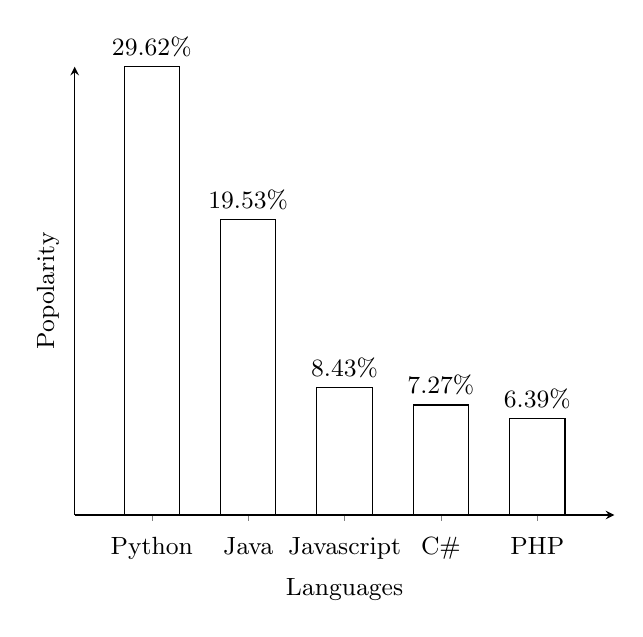
\begin{tikzpicture}[font=\small]
    \begin{axis}[
      ybar,
      bar width=20pt,
      xlabel={Languages},
      ylabel={Popolarity},
      ymin=0,
      ytick=\empty,
      xtick=data,
      axis x line=bottom,
      axis y line=left,
      enlarge x limits=0.2,
      symbolic x coords={Python,Java,Javascript,C\#,PHP},
      xticklabel style={anchor=base,yshift=-\baselineskip},
      nodes near coords={\pgfmathprintnumber\pgfplotspointmeta\%}
    ]
      \addplot[fill=white] coordinates {
        (Python,29.62)
        (Java,19.53)
        (Javascript,8.43)
        (C\#,7.27)
        (PHP,6.39)
      };
    \end{axis}
  \end{tikzpicture}
  \caption{Programming languages popularity}
  \label{lang}
\end{figure}

\section{Critical Analysis}
\label{analysis}
In this section is discussed which pro and cons the Ansible architecture has, and what should have be done to improve it.
\subsection{Pro}
\subsubsection{Easy to learn}
Users can easy catch up on how Ansible works and increase their productivity by a lot. The documentation is clear, full of examples, and in a short amount of time one can be a good Ansible user. With pretty much no dependendencies, the installation is immediate and the results of each task against whom clearly explain what happend, making it easy to debug.
\subsubsection{Agentless}
For managing the nodes Ansible relies on SSH, and in his way it doesn't require any agents to be installed on remote systems, which means less maintence ovehead and again, an easy deploy.
\subsubsection{Yaml}
Ansible has to be human readable, and almost all of its configurations are writable in Yaml, which configuration management and automation purposes is a better fit than other formats, as JSON, or programming languages or even worst, an had hoc language. Many of its competitor decided to use the latter.
\subsubsection{Opensource}
All its code is opensource, deployed on \textit{Github}, and is community driven. This means that everyone can make a pull request with a new feature, and if its main developers find it usefull and follow the Ansible goal, can be developed next from its mantainers.
\subsubsection{Modularity}
If Ansible lacks of a module or a plugin, is common to create a custom one and to merge it with the others. It just has some simply requirements, for example a module must return a json file and, and a plugin must be written in python. Other than that, every team can upgrade its own version of Ansible following the company desires.
\subsection{Cons}
\subsubsection{CLI}
Ansible doesn't have a GUI. For many this can be a problem, but Ansible was designed to have only a command-line interface. The configuration files this way can be modified using the prefered text editor, for example \textit{vim} or \textit{sublime-text}. \textit{Ansible Tower} was created to compensate this lack, but it still has much room for improvement. Only 85\% Ansible features are supported and is quite common to fall out of sync with the command line.
\subsubsection{Almost no Window support}
When Ansible was born, it supported only Unix nodes. After version 1.7 it started to support Windows nodes, using the native powershell remoting, but it still require a Unix control machine for managing hosts.
\subsubsection{Young}
Differently from its competitor, Ansible is much younger. Because of that, it has a smaller developer and user communitity, with the lowest material on the web for self-help and troubleshooting comparing to its competitors. For that reason is more common that Ansible has undocumented bugs. 
\subsubsection{SSH}
Ansible relies on SSH to push its modules and complete the tasks. This can be a problem if the SSH connection isn't a solid one. If SSH fails, then the execution fails; if the SSH connection is slow, then the execution is slow. For this reason, users must be very carefull about IP rules, LDAP and fail2ban configurations on their nodes.

\section{Similar Architectures}
\label{similar}
There are other tools that aim to the same goal as ansible: deploy, configure and manage nodes.
The most popular ones, that compete with Ansible for the same users, are
\begin{itemize}
    \item Chef
    \item Puppet
    \item Saltstack
\end{itemize}
The drives behind them are similar, but not the same. There are many differencies between them, and a good devops engineer must choose the best one for its needs, evaluating pro and cons of each architecture.
\subsection{Differences}
\subsubsection{Chef}
Chef has a master-agent architecture: the chef server runs on the master machine, and the chef clients run as an agent on each node. There is even another different component, the worstation, which contains all the configurations that are tested before pushing them to the central chef server.\\
If the chef server fails, it has a backup server to take place of the primary server, having a system with a minimum of fault tollerance.\\
Configuration files are made in Ruby DSL, a programming language that exploits the possibility to Ruby to be a metaprogramming languages, and for this reason the user must be a programmer to be able to configure it.\\
The chef server must be run on a Unix machine, but clients and the workstation can be run on every operating system.\\
\subsubsection{Puppet}
Puppet has a master-agent architecture: the puppet server runs on the master machine, and the puppet clients run as an agent on each node. There is a certificate signing between them, and for this reason the deploy is not fast.\\
Having a multi-master architecture, if the active master crashes, is elected another leader that its place.\\
Puppet has is own language, called Puppet DSL, in which the engineer has to know and masters before being able to create a proper configuration. Each client pulls the configuration from the master.\\
The puppet server must be run on a Unix machine, but clients work on every operating system.\\
\subsubsection{Saltstack}
Saltstack has a master-agent architecture: the salt master runs on the master machine, and the salt minions run as an agent on each node.\\
In the default mode, it has only one salt master, but it can be configured to have multiple masters. If the first master goes down, then the clients try to retrieve the configuration from the next in line.\\
Like Ansible, it use the YAML syntax, making it quite easy to understand and master.\\
The saltstack server must be run on a Unix machine, but clients work on every operating system.\\

\section{Conclusions}
Is possible to say that Ansible has a well designed architecture, with the lowest installation and deploy time, compared to its competitor, and with the simplest configuration syntax, having adopted YAML instead of a custom language.\\ Its main flaws are the lack of a GUI for its users and its young state. The simple but powerfull architecture allows to devops engineers to personalize at a granular level the configuration of their system.


\begin{thebibliography}{}
\label{references}
\bibitem{b1}P.Masek, M. Stusek, J. Krejci, K. Zeman, J. Pokorny, M. Kudlacek, ''Unleashing Full Potential of Ansible Framework: University Labs Administration'', IEEE, Jyvaskyla, Finland, 5-18 May 2018, [2018 22nd Conference of Open Innovations Association (FRUCT)].
\bibitem{b2}G. Violettas, S. Petridou, L. Mamatas, ''Routing under Heterogeneity and Mobility for the Internet of Things: A Centralized Control Approach'', IEEE, Abu Dhabi, United Arab Emirates, 9-13 Dec. 2018, [2018 IEEE Global Communications Conference (GLOBECOM)].
\bibitem{b3}W. Yiran, Z. Tongyang, G. Yidong, ''Design and implementation of continuous integration scheme based on Jenkins and Ansible'', IEEE, Chengdu, China, 26-28 May 2018, [2018 International Conference on Artificial Intelligence and Big Data (ICAIBD)].
\bibitem{b4}N. K. Singh, S. Thakur, H. Chaurasiya, H. Nagdev, ''Automated provisioning of application in IAAS cloud using Ansible configuration management'', IEEE, Dehradun, India, 4-5 Sept. 2015, [2015 1st International Conference on Next Generation Computing Technologies (NGCT)].
\bibitem{b5}V. Shvetcova, O. Borisenko, M. Polischuk,''Domain-Specific Language for Infrastructure as Code'', IEEE, Velikiy Novgorod, Russia, 13-14 Sept. 2019, [2019 Ivannikov Memorial Workshop (IVMEM)].
\bibitem{b6}J. Keating, ''Mastering Ansible'', Packt Publishing Ltd., Birmingham, Nov. 2015, pp 1-33.
\bibitem{b7}A. Patawari, V. Aggarwal, ''Ansible 2 Cloud Automation Cookbook'', Packt Publishing Ltd., Birmingham, Feb. 2018, pp 15-23,155-165.
\bibitem{b8}"Ansible Documentation", Accessed on: Nov. 25, 2019, [Online], Avaible: \href{https://docs.ansible.com/ansible/latest/index.html}{https://docs.ansible.com/ansible/latest/index.html} .
\bibitem{b9}"Ansible Source Code", Accessed on: Nov. 25, 2019, [Online], Avaible: \href{https://github.com/ansible/ansible}{https://github.com/ansible/ansible} .
\end{thebibliography}

\end{document}
